\chapter{Avaliação empírica}
\label{sec:avaliacao-empirica}

Nesse capítulo faremos experimentos comparativos para avaliar a eficiência do algoritmo de conexidade dinâmica elaborado no Capítulo~\ref{sec:connDG}. Como esse algoritmo foi desenvolvido  por Holm, de Lichtenberg e Thorup, ele é conhecido na literatura pelo acrônimo~\HDT.

O principal algoritmo concorrente foi desenvolvido por Henzinger e King~\cite{HenzingerKing} e é denotado por~\HK.
Ele empata o consumo assintótico amortizado esperado de $\O{\lg^2 n}$ de~\HDT.

Ambos os algoritmos visam manter uma floresta maximal geradora do grafo dinâmico para realizar o teste de conexidade e usam a mesma estratégia de atribuir níveis às arestas do grafo para amortizar o custo das operações.

A principal diferença entre eles é que~\HK{} sorteia arestas reservas e as testa para verificar se substituem uma aresta removida da MSF. Portanto seu consumo de tempo é necessariamente esperado, enquanto que~\HDT{} pode ser completamente determinístico se a implementação das florestas dinâmicas usadas for determinística. 

\section{Estudos anteriores}

Em $2010$, Tarjan e Werneck~\cite{tarjanWerneck2010} fizeram um estudo experimental com diversas estruturas de dados que solucionam o problema de conexidade para florestas dinâmicas.
Destacando diferentes qualidades e deficiências de cada estrutura de dados quando sujeitas a diferentes tipos de cargas de trabalho.
Os autores concluem que as link-cut trees tiveram a melhor performance geral.

Para apresentar os estudo experimentais que abordam conexidade em grafos dinâmicos, usaremos a revisão histórica apresentada por~\cite{Zaroliagis2002}.

O primeiro estudo experimental que trata sobre o problema de conexidade em grafos dinâmicos data de~$1997$ e foi feito por Alberts, Cattaneo, e Italiano~\cite{EmpiricalStudy1997}.
Esse estudo não analisa~\HDT{} e somente compara~\HK{} com um algoritmo desenvolvido por~Eppstein et al.~\cite{Eppstein1992SparsificationaTF} que utiliza uma técnica chamada esparsificação para reduzir o custo assintótico das operações aplicadas ao grafo para~$\O{\!\sqrt{n}}$.
Ambos os algoritmos foram implementados em~C++.

O estudo conclui que~\HK{} se torna mais eficiente do que o algoritmo de Eppstein et al. quando o número de atualizações aplicadas a um grafo dinâmico é aproximadamente duas vezes o número de vértices do grafo. Esse fenômeno é devido à amortização utilizada por~\HK{}, que necessita de um número razoável de atualizações para diluir o custo das operações. 

A partir da implementação de~\HK{} fornecida por esses autores, em $2002$, Raj Iyer, David Karger, Hariharan Rahul e Mikkel Thorup~\cite{EmpiricalStudy2002} implementaram \HDT{} e o compararam com~\HK{}.

A implementação de~\HDT{} que esses autores fornecem inclui algumas heurísticas. Dentre elas, sortear arestas reservas e verificar se são substitutas de uma aresta removida antes de realizar a busca determinística~\cite[Seção 4.1]{EmpiricalStudy2002}.
Essa heurística se baseia na maneira como~\HK{} busca arestas substitutas e os autores decidiram utilizá-la, pois notaram que com poucos sorteios se encontrava uma aresta substituta. 
Nesse estudo os autores concluem que~\HK{} é dominado por~\HDT{}



Em $2022$, Chen et al.\cite{QC22} propõem uma heurística para garantir baixo consumo de tempo da consulta de conexidade e, para mostrar a eficiência dessa heurística, realizam um estudo empírico comparando sua solução com~\HK{} implementadas em Python~$3$.
Chamaremos esse algoritmo heurístico de~\CLHB{} e elaboraremos mais sobre ele na próxima seção.



\section{Escopo}

Em nosso experimento, faremos testes com conjuntos de dados reais.
Compararemos~\HDT{} com a implementação de~\HK{} apresentada por Chen~et al.~\cite{QC22}.
No entanto não incluiremos o algoritmo desenvolvido por esses autores em nosso experimento.

Como comentado anteriormente, a solução desenvolvida por Chen~et al. se baseia na heurística de que grafos reais possuem baixo diâmetro.
Para concluir isso, os autores analisaram~$1324$ grafos presentes em um banco de dados~\cite{KONECT} e notaram que~$1185$ deles possuem diâmetro menor do que~$16$.
Com essa informação, eles desenvolveram uma estrutura de dados que possui consumo de tempo linear em função do diâmetro do grafo,
portanto se beneficiando desse baixo diâmetro empiricamente observado.

Na Figura~\ref{fig:sensibilidade-diametro} podemos observar um gráfico que mostra o consumo de tempo de consulta de conexidade em \HK{}, \HDT{} e~\CLHB{} em função do diâmetro do grafo que está sendo operado.

\begin{figure}
\begin{tikzpicture}
    \begin{axis}[
		 ylabel=consumo de consulta de conexidade (s),
		 xlabel=Diâmetro~$D$,
		 width=0.5\linewidth,
	         ]
    \addplot[orange] table [x=avg_sp, y=Dtree, col sep=comma] {csv/avg_sp.csv};
    \addlegendentry{\CLHB}
    \addplot[black] table [x=avg_sp, y=HK, col sep=comma] {csv/avg_sp.csv};
    \addlegendentry{\HK}
    \addplot[blue] table [x=avg_sp, y=HDT, col sep=comma] {csv/avg_sp.csv};
    \addlegendentry{\HDT}
\end{axis}
\end{tikzpicture}
\caption{Consumo de tempo de consulta de conexidade em função do diâmetro do grafo.}
\label{fig:sensibilidade-diametro}
\end{figure}

No entanto, analisando esse mesmo banco de dados, notamos que dos~$1324$ grafos presentes nesse banco de dados, $1015$ vêm de uma única fonte -- 
propriamente dita, são provenientes da Wikimedia~\cite{wikimedia}, responsável pela Wikipédia e afins -- 
e $809$ destes grafos são classificados na mesma categoria, isto é, grafos bipartidos que relacionam autores com paginas web editadas por eles. Como há poucos autores em relação ao número de páginas web, o diâmetro de cada componente conexa desses grafos tende a ser baixo.

Se excluirmos esses~$1014$, a quantidade de grafos com diâmetro estritamente menor do que~$16$ diminui para~$63\%$, como mostra a Figura~\ref{fig:distdiametro}.
Uma cifra muito menos relevante do que os~$89\%$ incluindo os grafos providos pela Wikimedia.

\begin{figure}
\begin{center}
\begin{tikzpicture}
    \begin{axis}[
         ybar,
	 ylabel=$\%$ de grafos com diâmetro $D$,
         xlabel=Diâmetro $D$,
         symbolic x coords={1--5,6--10,11--16,17--20,20+},
         legend pos=north east,
         nodes near coords,
         title={Distribuição de diâmetros}
	 ]
    \addplot[fill=blue] table [x=intervalo,col sep=comma] {csv/data-analysis/non-wiki-grafico-resumido.csv};
    %\addlegendentry{s/ wikimedia}
    \addplot[fill=orange] table [x=intervalo,y=wiki,col sep=comma] {csv/data-analysis/non-wiki-grafico-resumido.csv};
    %\addlegendentry{c/ wikimedia}
\end{axis}
\end{tikzpicture}
\caption{Em laranja, mostramos a distribuição de diâmetros no banco de dados~\cite{KONECT}. Em azul, a mesma distribuição excluindo grafos originários da Wikimedia.}
\label{fig:distdiametro}
\end{center}
\end{figure}

Além disso, observamos uma tendência de grafos que representam infraestruturas físicas (como rodovias, rotas aéreas e malha energética) possuírem diâmetro muito maior do que~$16$.
O que indica que a eficiência de~\CLHB{} está fortemente ligada ao contexto em que é utilizado. 

Como a proposta desse trabalho é analisar soluções adequadas para uso geral, independente de contexto ou características especificas dos grafos utilizados, não consideramos adequado incluir~\CLHB{} em nosso estudo comparativo.


Dessa forma, somente compararemos~\HK{} com~\HDT{} e para fazer isso usaremos os grafos listados na Tabela~\ref{tab:datasets}.
Todos os grafos foram retirados do NetworkRepository~\cite{nr-aaai15}, um grande repositório de grafos.


\begin{table}
\begin{center}
\begin{tabular}{ |c|c|c|c| } 
 \hline
	Nome & $|V|$ & $|E|$ & N° de atualizações\\
 \hline
	email-dnc (DNC)&$1.9\times 10^3$&$3.74\times 10^4$&$3.2\times 10^4$\\
 \hline
	Call (CA)&$7\times 10^3$&$5.1\times 10^4$&$2.3\times 10^4$\\
 \hline
	messages (MS)&$2\times 10^3$&$6\times 10^4$&$6.3\times 10^4$\\
 \hline
	FB-FORUM (FB)&$8.99\times 10^2$&$3.5\times 10^4$&$3.8\times 10^4$\\
 \hline
	Wiki-elec(WI)&$7.1\times 10^3$&$1.07\times 10.5$&$2.1\times 10^5$\\
 \hline
	tech-as-topology(Tech)&$3.4\times 10^4$&$1.71\times 10^5$&$2.7\times 10^5$\\
 \hline
	Enron(EN)&$8.7\times 10^4$&$1.1\times 10^6$&$1.28\times 10^6$\\
 \hline
\end{tabular}
\caption{Grafos dinâmicos retirados de~\cite{nr-aaai15}}
\label{tab:datasets}
\end{center}
\end{table}


\section{Metodologia}

\cite{guideXP1999}

\section{Resultados}

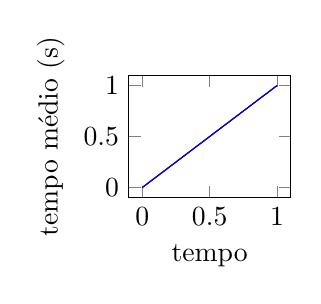
\begin{tikzpicture}
    \begin{axis}[
		 ylabel=tempo médio (s),
		 xlabel=tempo,
		 width=0.3\linewidth,
	         ]
    \addplot[orange,domain=0:1]{x};
    \label{pgfplots:Dtree:QueryCall}
    \addplot[black,domain=0:1]{x};
    \label{pgfplots:HK:QueryCall}
    \addplot[blue,domain=0:1]{x};
    \label{pgfplots:HDT:QueryCall}
    \end{axis}
\end{tikzpicture}


\newpage

\subsection{Inserção de aresta reserva}
\legenda
\begin{figure}
\tabela{csv/call/updates/call_insertion_nte.csv}{Call}{insertionCall}
\tabela{csv/dnc/updates/dnc_insertion_nte.csv}{DNC}{QueryDNC}
\tabela{csv/enron/updates/enron_insertion_nte.csv}{EN}{QueryENRON}
\tabela{csv/fb/updates/fb_insertion_nte.csv}{FB}{QueryFB}
\tabela{csv/messages/updates/messages_insertion_nte.csv}{MS}{QueryMS}
%\tabela{csv/tech/updates/tech_insertion_nte.csv}{Tech}{QueryTech}
\tabela{csv/wiki/updates/wiki_insertion_nte.csv}{WI}{QueryWiki}
\caption{Performance de inserção de arestas reservas}
\end{figure}



\newpage
\subsection{Inserção de aresta da árvore}
\legenda
\begin{figure}
\tabela{csv/call/updates/call_insertion_te.csv}{Call}{insertionCall}
\tabela{csv/dnc/updates/dnc_insertion_te.csv}{DNC}{QueryDNC}
\tabela{csv/enron/updates/enron_insertion_te.csv}{EN}{QueryENRON}
\tabela{csv/fb/updates/fb_insertion_te.csv}{FB}{QueryFB}
\tabela{csv/messages/updates/messages_insertion_te.csv}{MS}{QueryMS}
%\tabela{csv/tech/updates/tech_insertion_te.csv}{Tech}{QueryTech}
\tabela{csv/wiki/updates/wiki_insertion_te.csv}{WI}{QueryWiki}
\caption{Performance de inserção de arestas da árvore}
\end{figure}

\newpage
\subsection{Remoção de aresta reserva}
\legenda
\begin{figure}
\tabela{csv/call/updates/call_insertion_nte.csv}{Call}{insertionCall}
\tabela{csv/dnc/updates/dnc_deletion_nte.csv}{DNC}{QueryDNC}
\tabela{csv/enron/updates/enron_deletion_nte.csv}{EN}{QueryENRON}
\tabela{csv/fb/updates/fb_deletion_nte.csv}{FB}{QueryFB}
\tabela{csv/messages/updates/messages_deletion_nte.csv}{MS}{QueryMS}
%\tabela{csv/tech/updates/tech_deletion_nte.csv}{Tech}{QueryTech}
\tabela{csv/wiki/updates/wiki_deletion_nte.csv}{WI}{QueryWiki}
\caption{Performance de inserção de arestas reservas}
\end{figure}


\newpage
\subsection{Remoção de aresta da árvore}
\legenda
\begin{figure}
\tabela{csv/call/updates/call_insertion_te.csv}{Call}{insertionCall}
\tabela{csv/dnc/updates/dnc_deletion_te.csv}{DNC}{QueryDNC}
\tabela{csv/enron/updates/enron_deletion_te.csv}{EN}{QueryENRON}
\tabela{csv/fb/updates/fb_deletion_te.csv}{FB}{QueryFB}
\tabela{csv/messages/updates/messages_deletion_te.csv}{MS}{QueryMS}
%\tabela{csv/tech/updates/tech_deletion_te.csv}{Tech}{QueryTech}
\tabela{csv/wiki/updates/wiki_deletion_te.csv}{WI}{QueryWiki}
\caption{Performance de inserção de arestas da árvore}
\end{figure}


\newpage
\subsection{Consulta de conexidade}
\legenda
\begin{figure}
\tabela{csv/call/query_call.csv}{Call}{QueryCall}
\tabela{csv/dnc/query_dnc.csv}{DNC}{QueryDNC}
\tabela{csv/enron/query_enron.csv}{EN}{QueryEN}
\tabela{csv/fb/query_fb.csv}{FB}{QueryFB}
\tabela{csv/messages/query_messages.csv}{MS}{QueryMS}
%\tabela{csv/tech/query_tech.csv}{Tech}{QueryTech}
\tabela{csv/wiki/query_wiki.csv}{WI}{QueryWiki}
\caption{Performance da consulta de conexidade}
\end{figure}

\newpage
\subsection{Soma das distâncias de nós até suas raizes}
Para cada vértice~$v$ no grafo, é calculado a distância~$D_v$ do nó que representa esse vértice até a raiz da ABB.
Em seguida é feita a soma de todos os~$D_v$.

\legenda
\begin{figure}
\tabela{csv/call/Sd_call.csv}{Call}{QueryCall}
\tabela{csv/dnc/Sd_dnc.csv}{DNC}{QueryDNC}
\tabela{csv/enron/Sd_enron.csv}{EN}{QueryEN}
\tabela{csv/fb/Sd_fb.csv}{FB}{QueryFB}
\tabela{csv/messages/Sd_messages.csv}{MS}{QueryMS}
\tabela{csv/wiki/Sd_wiki.csv}{WI}{QueryWiki}
\caption{Performance da consulta de conexidade}
\end{figure}

